% The boundary conditions for the off-shore pipeline were inlet mass flow, outlet pressure, inlet temperature and inlet \co-concentration, see \cref{fig:offshorePipelineBC} for a plot of these. 
% The pipeline was simulated for a 14 day winter period and a 18 day summer period. 
% For the heat transfer model, sea bottom temperature and air temperature profiles along the pipeline that were sampled once per day were used as boundary conditions. The ambient sea bottom temperatures are from oceanographic models, and the air temperatures are expected temperatures based on historical measurements. \todo{Plot amb temp? 1 line per day, doable in 1 fig}


In \cref{fig:baseCaseWithZ} is a plot of the boundary conditions for the base case, and the results for a simulation where the compressibility factor $Z$ has been increased by \SI{20}{\percent}. 

% The biggest impact is on the inlet pressure, which is increased by up to \SI{7}{\percent}.

%In a simulation of a real pipeline, where measurements of the pressure etc. at the inlet and outlet are available, the pipeline roughness $\epsilon$ would typically have been tuned to match the measured pressure drop \todo{using data from a period of stable operation}. Here we have not tuned the roughness to match the base case pressure drop
% \begin{figure}[ht]%
%     \centering%
%     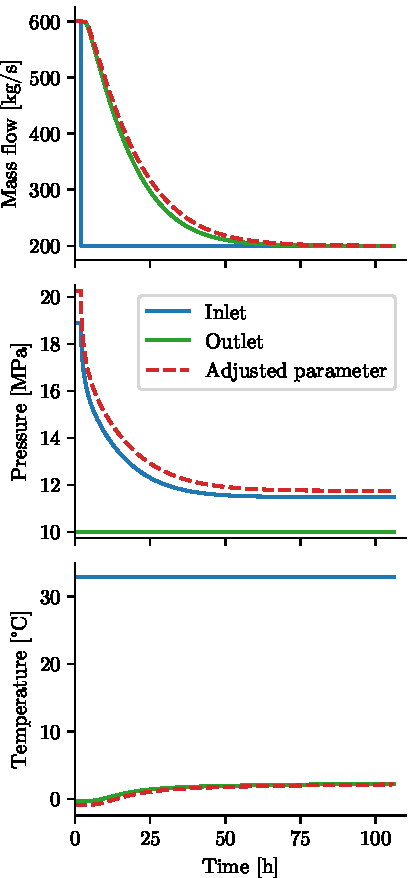
\includegraphics{figures/base_case_with_adjusted_Z.pdf}%
%     \caption{%
%         \redtext{Caption.} Inlet flow ramp down at 2 hours. Differences vary with time.
%         \label{fig:baseCaseWithZ}%
%     }%
% \end{figure}%
\begin{figure}[!ht]%
    \centering%
    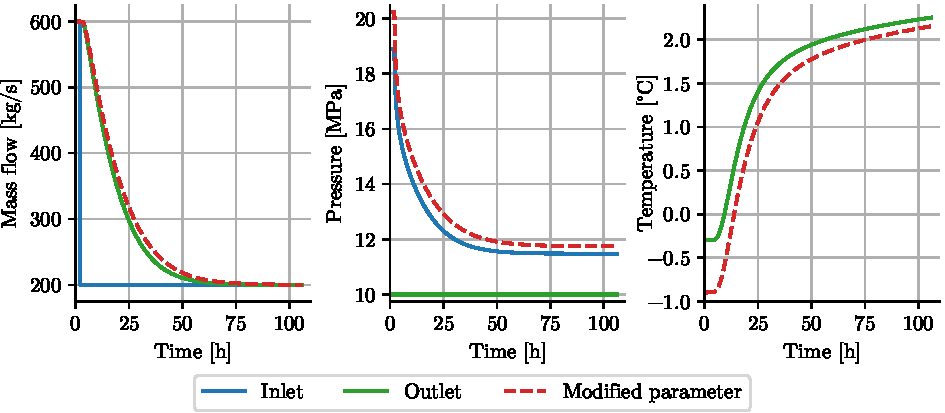
\includegraphics{figures/base_case_with_adjusted_Z_horiz.pdf}%
    \caption{%
        A plot of the results from the base case, and from a simulation with a modified parameter (the compressibility factor $Z$). The inlet flow rate transient occurs at 2~hours, and the boundary conditions are then kept constant for 104~hours. The constant inlet temperature of \SI{33}{\celsius} is not shown.
        \label{fig:baseCaseWithZ}%
    }%
\end{figure}%
From \cref{fig:baseCaseWithZ} it is clear that the difference between the base case and the cases with a modified parameter vary with time during the transient%
, so to more easily analyze the results, both the time average relative difference
\begin{align}
    &\overbar{\Delta y_\mathrm{rel}}
    = \frac{1}{n} \sum_{i=1}^n \Delta y_{\mathrm{rel}, i}
    = \frac{1}{n} \sum_{i=1}^n \frac{y_i - y_i^0}{y_i^0},
    &\text{where}~n~\text{is the number of time steps,}
\end{align}
and the maximum relative difference
\begin{align}
    \max\del{\Delta y_\mathrm{rel}} = \max\del{\frac{y_i - y_i^0}{y_i^0}}
\end{align}
between the base case ($y^0$) and the simulations with modified parameters ($y$) was calculated, for mass flow, pressure and temperature. %
This was calculated for each parameter in the sensitivity study, at every grid point in the simulations. Since a transient case is simulated, and both the temperature and the pressure vary between the inlet and the outlet, relative differences are used. %
% For for mass flow and pressure the relative difference was used
% \begin{align}
%     \eval{\Delta y}_\textrm{relative} = \frac{y - y^0}{y^0}
% ,
% \end{align}
% while the absolute difference was used for temperature
% \begin{align}
%     \eval{\Delta y}_\textrm{absolute} = \abs{y - y^0}
% .
% \end{align}
%
% A plot of the maximum and average differences for the compressibility factor $Z$ can be seen in \cref{fig:maxAndAverageDiffForZ}, where the maximum and average mass flow, pressure, and temperature difference is shown for the whole pipeline. 
%
A plot of the maximum and average differences as function of position, for all parameters in the study, are shown in \cref{fig:maxAndAverageForAll}, and a list of the average impact on the whole pipeline is given in \cref{tab:averageImpact}. %

From \cref{fig:maxAndAverageForAll} a) and b) it can be seen that the parameters with the highest impact on both mass flow and pressure are the friction factor $f$ and the compressibility factor $Z$. For the mass flow the greatest impact is at the outlet, with a gradual decrease from the inlet to the outlet. For the pressure the situation is reversed. This behaviour is caused by how the simulations are set up, with the inlet mass flow and the outlet pressure as boundary conditions.
% All other parameters have %
% less than \SI{1.3}{\percent} maximum %
% %(\redtext{1.23 for dZdT|p}) %
% and less than \SI{0.3}{\percent} average %
% %(\redtext{0.278 for dZdp|T}) %
% impact on the mass flow, and %
% less than \SI{0.5}{\percent} maximum %
% % (\redtext{0.471 for viscosity}) %
% and \SI{0.4}{\percent} average %
% % (\redtext{0.337 for viscosity}) %
% impact on the pressure. %

The average impact for the whole pipeline was calculated by averaging over the time averaged difference for each grid point. %, $\overbar{\Delta y_{\mathrm{rel},j}}$. %
% using a weighted average, since we use non-uni
% \begin{align}
%     &\frac{1}{L}\sum_{j=1}^{m}\frac{1}{2} 
%     \del{\overbar{\Delta y_\mathrm{rel}}_{,j} + \overbar{\Delta y_\mathrm{rel}}_{,j+1}} \Delta x_i
%     , &\text{where}~m~\text{is the number of grid points.}
% \end{align}
A list of the average impact of all parameters is listed in \cref{tab:averageImpact}. %
%
The average impact on mass flow is found to be \SI{1.43}{\percent} for the friction factor and \SI{0.90}{\percent} for the compressibility factor, % 6.5703443811 4.133998237
which is respectively 6.6 and 4.1 times higher than the third most important factor, $\eval{\partial Z/\partial p}_T$, which has an average impact of \SI{0.22}{\percent}. %
%
The average impact on pressure is \SI{3.09}{\percent} for the friction factor and \SI{2.07}{\percent} for the compressibility factor, % 14.3347939844 9.6177252345
which is respectively 14.3 and 9.6 times higher than the third most important factor, the viscosity $\mu$, which has an average impact of \SI{0.22}{\percent}. %
%
% Further, peaks in several of the mass flow and temperature responses are seen between where the pipeline enters the ocean at \SI{25}{\kilo\meter} and \SI{50}{\kilo\meter}.

\begin{figure}[!p]%
    \centering%
    % 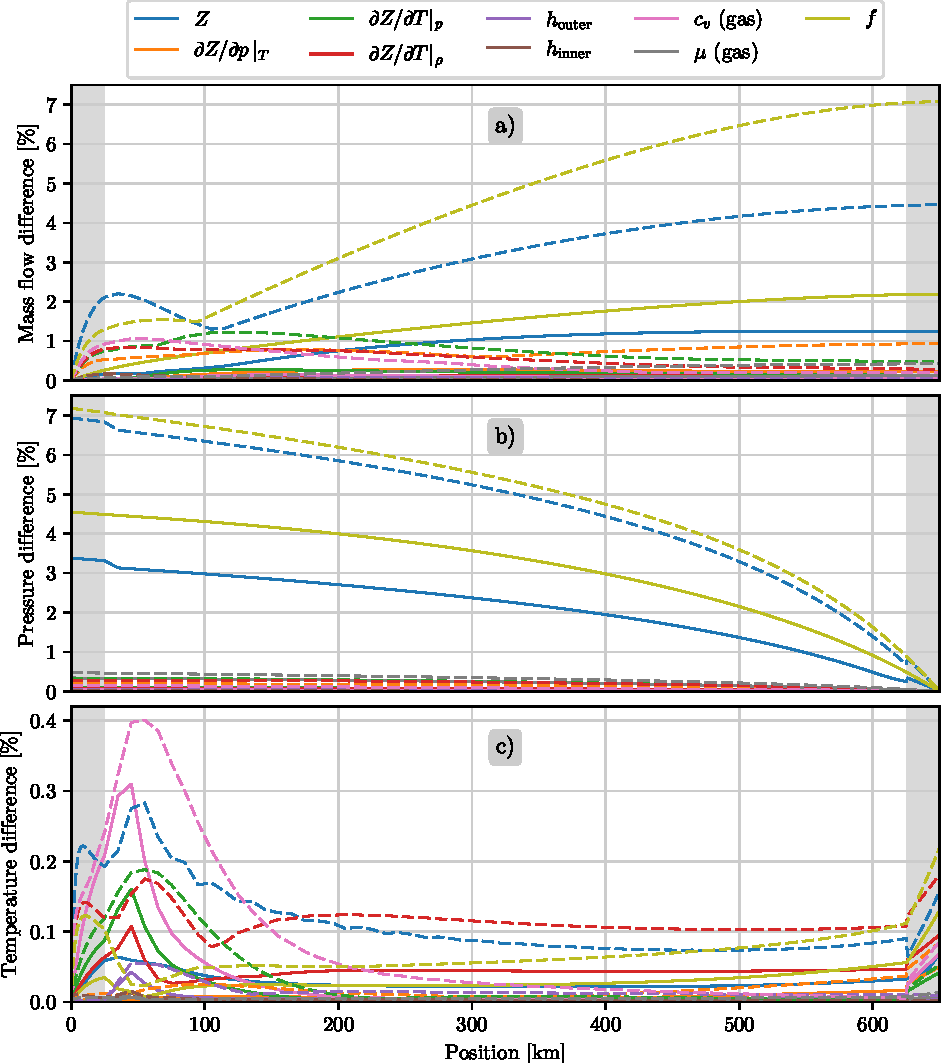
\includegraphics{figures/difference_along_pipeline_shaded_abc.pdf}%
    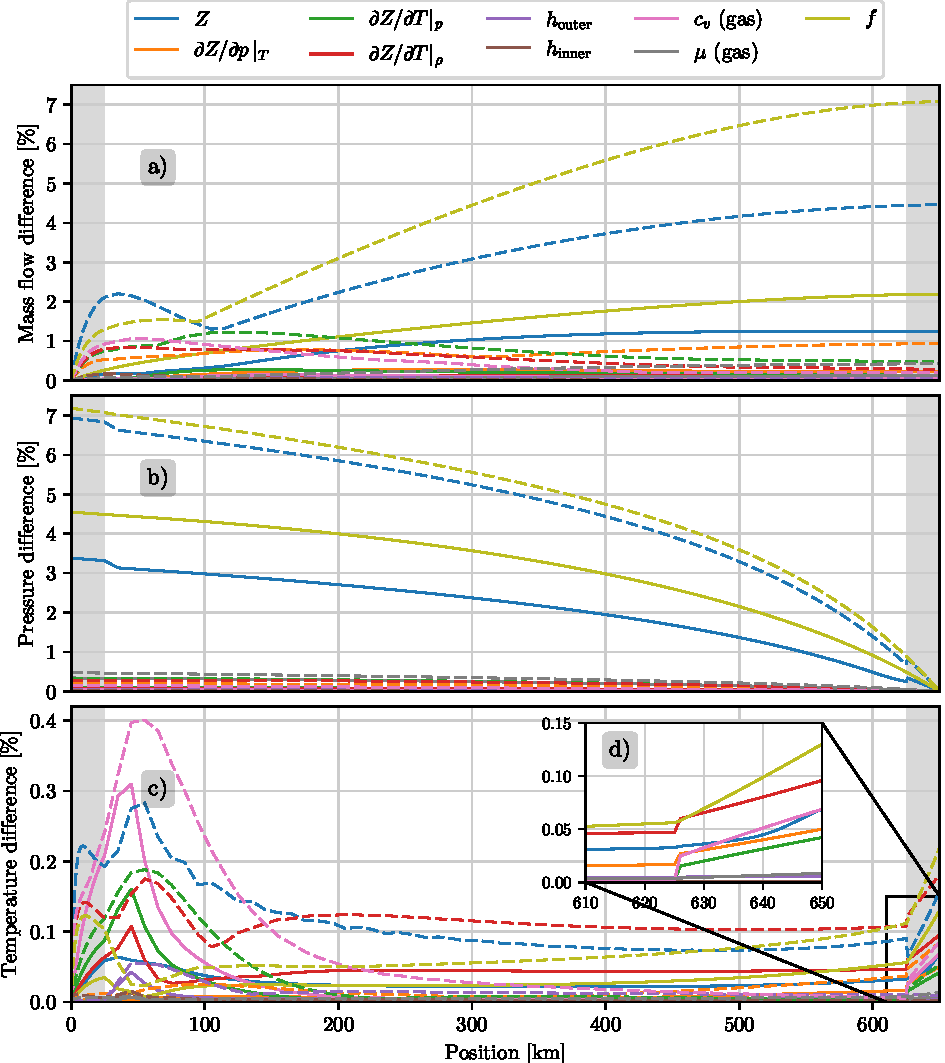
\includegraphics{figures/difference_along_pipeline_shaded_abc_inset.pdf}%
    \caption{%
        Plots of the maximum (dashed lines) and time average (solid lines) difference between the base case and the cases with a parameter increased by \SI{20}{\percent}, for each grid point used in the simulations. The gray shaded areas on the left and right side illustrate the on-shore parts of the pipeline.
        \label{fig:maxAndAverageForAll}%
    }%
\end{figure}%

\begin{table}[!hb]
    \caption{
        Table of the average relative difference in mass flow, pressure and temperature, for all parameters in the sensitivity study. 
        % \redtext{weighted average using non-uniform grid spacing} %
        % For mass flow and pressure the two highest numbers are highlighted in green, and the third-highest in yellow.
        \label{tab:averageImpact} %
    } %
    % \begin{tabular}{lc}
    \centering %
    % \begin{tabular}{lS}
    \begin{tabular}{cccc} %
        \toprule
        % Parameter & \parbox{3.3cm}{\centering Average \\ difference in \\ mass flow [\si{\percent}]} & \parbox{3.3cm}{\centering Average \\ difference in \\ pressure [\si{\percent}]} & \parbox{3.3cm}{\centering Average \\ difference in temperature [\si{\percent}]} \\
        & \multicolumn{3}{c}{Average relative difference} \\ \cmidrule(r){2-4}
        \parbox{2.5cm}{\centering Parameter} & Mass flow [\si{\percent}] & Pressure [\si{\percent}] & Temperature [\si{\percent}] \\
        \midrule
        % output from Python script goes here
        % relative temperature
        $Z$ & 0.9007 & 2.0722 & 0.0289 \\
        $\eval{\partial Z/\partial p}_T$ & 0.2179 & 0.0527 & 0.0084 \\
        $\eval{\partial Z/\partial T}_p$ & 0.1859 & 0.0614 & 0.0157 \\
        $\eval{\partial Z/\partial T}_\rho$ & 0.1021 & 0.0567 & 0.0454 \\
        $h_\mathrm{outer}$ & 0.0171 & 0.0073 & 0.0061 \\
        $h_\mathrm{inner}$ & 0.0033 & 0.0015 & 0.0015 \\
        $c_v$ (gas) & 0.0881 & 0.0225 & 0.0321 \\
        $\mu$ (gas) & 0.0782 & 0.2155 & 0.0027 \\
        $f$ & 1.4316 & 3.0885 & 0.0306 \\
        \bottomrule
    \end{tabular}
\end{table}

% % \begin{table}[ht]
%     \begin{center}
%         \begin{tabular}{RRRRRRRRRR}
%           1.00 & 1.00 & 1.00 & 1.00 & 0.99 & 0.98 & 0.96 & 0.90 & 0.82 & 0.37 \\
%           1.00 & 1.00 & 0.99 & 0.98 & 0.95 & 0.90 & 0.82 & 0.61 & 0.37 & 0.01 \\
%           1.00 & 0.99 & 0.98 & 0.96 & 0.90 & 0.82 & 0.67 & 0.37 & 0.14 & 0.00 \\
%           1.00 & 0.98 & 0.95 & 0.90 & 0.78 & 0.61 & 0.37 & 0.08 & 0.01 & 0.00 \\
%           0.99 & 0.95 & 0.90 & 0.82 & 0.61 & 0.37 & 0.14 & 0.01 & 0.00 & 0.00 \\
%           0.98 & 0.90 & 0.82 & 0.67 & 0.37 & 0.14 & 0.02 & 0.00 & 0.00 & 0.00 \\
%           0.95 & 0.78 & 0.61 & 0.37 & 0.08 & 0.01 & 0.00 & 0.00 & 0.00 & 0.00 \\
%           0.90 & 0.61 & 0.37 & 0.14 & 0.01 & 0.00 & 0.00 & 0.00 & 0.00 & 0.00 \\
%           0.82 & 0.37 & 0.14 & 0.02 & 0.00 & 0.00 & 0.00 & 0.00 & 0.00 & 0.00 \\
%           0.37 & 0.01 & 0.00 & 0.00 & 0.00 & 0.00 & 0.00 & 0.00 & 0.00 & 0.00 \\
%         \end{tabular}
%     \end{center}
% \end{table}

\begin{table}[!hb]
    \caption{
        \redtext{caption}
        \label{tab:}
    }
    \centering
    \begin{tabular}{lRRT}
        \toprule
         % & \multicolumn{3}{c}{Item} \\
        & \multicolumn{1}{c}{Chemical Component} \\% & \parbox{4cm}{\centering Average relative impact on pressure} & \parbox{4cm}{\centering Average impact on temperature} \\
        % Parameter & [\si{\percent}] & [\si{\percent}] & [\si{\celsius}] \\
        \midrule
        % output from Python script goes here
        $Z$ & 0.8058 & 1.9431 & 0.0925 \\
        $\eval{\partial Z/\partial p}_T$ & 0.1769 & 0.0483 & 0.0371 \\
        $\eval{\partial Z/\partial T}_p$ & 0.1414 & 0.0562 & 0.0749 \\
        $\eval{\partial Z/\partial T}_\rho$ & 0.0852 & 0.0503 & 0.1400 \\
        $h_\mathrm{seawater}$ & 0.0134 & 0.0064 & 0.0132 \\
        $h_\mathrm{inner}$ & 0.0030 & 0.0013 & 0.0035 \\
        $c_v$ (gas) & 0.0676 & 0.0214 & 0.1579 \\
        Viscosity & 0.0724 & 0.1985 & 0.0087 \\
        Friction & 1.3207 & 2.7952 & 0.1160 \\
        \bottomrule
    \end{tabular}
\end{table}

For the temperature the situation is less clear-cut. From \cref{tab:averageImpact} it is seen that the parameter which gives the highest average difference along the whole pipeline is the derivative of the compressibility factor $\eval{\partial Z/\partial T}_\rho$, with an average difference of \SI{0.045}{\percent}, 1.41~times the impact of the next parameter ($c_v$) and 1.48~times the impact of the third parameter ($f$). The effects on temperature are in general seen to be much smaller than for mass flow and pressure, and there are no parameters that stand out in the same way they for mass flow and pressure
% . Compared to mass flow and pressure, where the two parameters with the highest impact give a difference of between 4 and 14 times the parameter with the third highest impact, the numbers for the temperature seem to \redtext{vary less}.

In \cref{fig:maxAndAverageForAll} c), peaks in the temperature responses of up to \SI{0.31}{\percent} are observed around \SI{20}{\kilo\meter} off-shore, before the impact of all parameters steadily decrease until they stabilize around \SIrange{100}{200}{\kilo\meter} off-shore. Also, between \SI{125}{\kilo\meter} (\SI{100}{\kilo\meter} off-shore) and landfall at \SI{625}{\kilo\meter}, all parameters have much lower impact than closer to the start of the pipeline; no parameter have a higher maximum impact than \SI{0.15}{\percent} or an average impact of more than \SI{0.06}{\percent}. %
The stable behaviour in this area is caused by the fixed sea temperature, which acts as a thermal reservoir, so after a long off-shore section the gas comes to a thermal equilibrium with the sea water, and the gas temperature is governed by the ambient temperature.
% This is because, after being transported offshore for some time, the gas comes to a thermal equilibrium with the ambient sea water. The sea has fixed temperature, and acts as a thermal reservoir, so after a long off-shore section the gas temperature will be governed by the ambient temperature, 
% and will be independent of any parameters that affect the heat exchange rate between the gas and the ambient (\redtext{as long as the heat exchange rate is different from zero})\todo{what about things like Joule Thompson?, are there other effects??}.

Finally, there is a steady increase in the impact on temperature between landfall and the outlet for most parameters. This is because the boundary condition for the thermal exchange between the gas and the ambient changes at landfall (the pipeline goes from being exposed to sea water to buried under ground), and the thermal equilibrium between the gas and the ambient is disturbed. %Here the parameters that affect the heat exchange, like the inner and outer heat transfer coefficients, will again come into play
%
Some details on the temperature response near the outlet can be seen in the inset in \cref{fig:maxAndAverageForAll} d). It is clear that some of the parameters that have very little effect on the temperature while off-shore, like the heat capacity $c_v$ and the derivative of the compressibility factor $\eval{\partial Z/\partial T}_p$, have a much higher effect after going on-shore, and on the final outlet temperature. The impact of the derivative of the compressibility increases from \SI{0.0012}{\percent} at \SI{625}{\kilo\meter} to \SI{0.042}{\percent} at the outlet, a factor of 12.9, and the heat capacity $c_v$ increases from \SI{0.0018}{\percent} at \SI{625}{\kilo\meter} to \SI{0.069}{\percent} at the outlet, a factor of 13.8. The trend in the plot indicates that the impact would be even bigger with a longer on-shore section. In general it is observed that the exposure to the sea seem to reduce the impact of changes in the model parameters on the temperature.

% \begin{figure}[!ht]%
%     \centering%
%     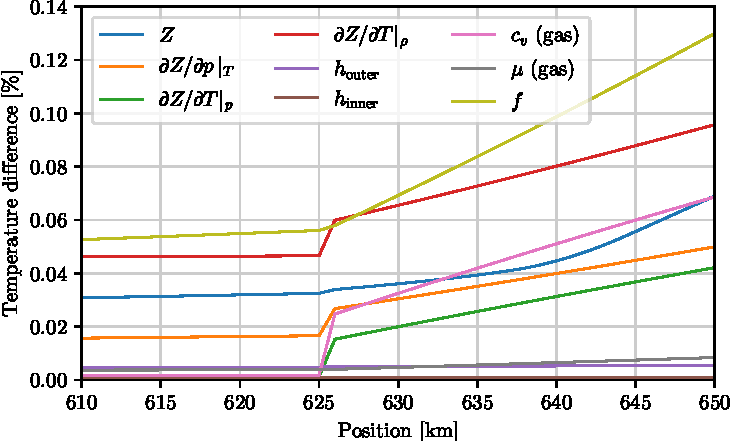
\includegraphics{figures/outlet_temperature_detail.pdf}%
%     \caption{%
%         Details of the response in temperature to changes in the different parameters, close to the outlet. Plot of the average temperature difference at each grid point.
%         % Plots of the maximum (dashed lines) and time average (solid lines) difference between the base case and the cases with a parameter increased by \SI{20}{\percent}. The gray shaded areas illustrate the on-shore parts of the pipeline.
%         \label{fig:outletTemperatureDetail}%
%     }%
% \end{figure}%

% \begin{figure}[!hb]%
%     \centering%
%     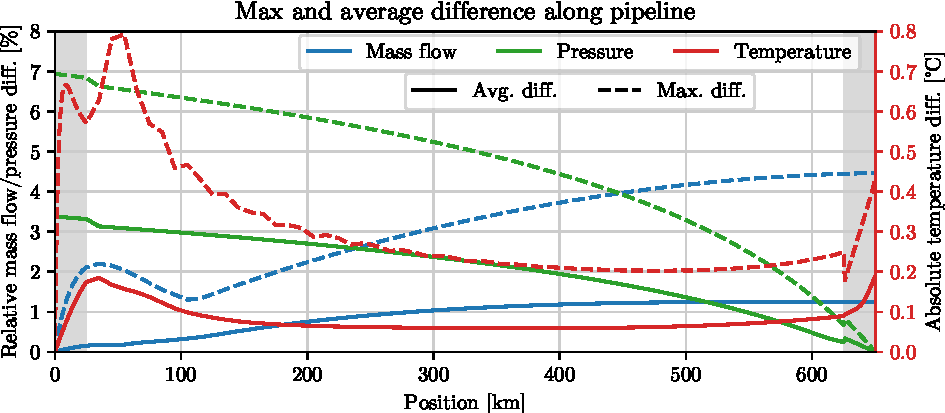
\includegraphics{figures/all_differences_position.pdf}%
%     \caption{%
%         The maximum (dashed lines) and time average (solid lines) difference between the base case and the results from the case with the compressibility factor $Z$ increased by \SI{20}{\percent}. Relative difference is used for mass flow and pressure (the left axis), and absolute difference for temperature (the right axis). The gray shaded areas illustrate the on-shore parts of the pipeline. \redtext{Not sure if this figure is necessary}
%         \label{fig:maxAndAverageDiffForZ}%
%     }%
% \end{figure}%

% In \cref{fig:massFlowBarChart,fig:pressureBarChart,fig:temperatureBarChart} the maximum and average differences between the base case and each case with modified parameters, at certain points of interest along the pipeline, are shown in bar charts. For the mass flow and pressure the observations from before are confirmed: the most important parameters are the friction factor $f$ and the compressibility factor $Z$, at the start of the pipeline for the pressure, and at the end of the pipeline for the mass flow.
%, like the inlet, the end of the on-shore section etc

To further analyze the temperature responses, the maximum and average temperature differences at certain points of interest along the pipeline are shown in a bar chart in \cref{fig:temperatureBarChart}. %
It is seen that the heat capacity $c_v$ is the parameter with the highest impact between all the selected points on the pipeline, with the two highest \emph{average} temperature differences (respectively at \SI{20}{\kilo\meter} off-shore, and at the end of the on-shore section), and the highest and third highest \emph{maximum} differences (respectively at \SI{20}{\kilo\meter} off-shore and at the end of the on-shore section). The parameter with the highest impact at \SI{300}{\kilo\meter} offshore is the derivative of the compressibility factor $\partial Z/\partial T\/|_\rho$, while at the end of the off-shore section and at the outlet it is the friction factor $f$.

% It can be seen that for the first 45 kilometers of the pipeline, the most important
% parameter is the heat capacity $c_v$, giving an average temperature difference of up to \SI{0.87}{\celsius} (maximum difference of \SI{1.14}{\celsius}). Following this, in descending order of importance are the derivatives of the compressibility %
% $\eval{\partial Z/\partial T}_p$ %
% % $\eval{\pd{Z}{T}}_p$%
%  and %
% $\eval{\partial Z/\partial T}_\rho$%
% % $\eval{\pd{Z}{T}}_\rho$%
% ; and finally the compressibility itself, $Z$, with
% average temperature difference of up to \SI{0.45}{\celsius} (maximum difference of \SI{0.78}{\celsius}). %

% \begin{figure}[!p]%
%     \centering%
%     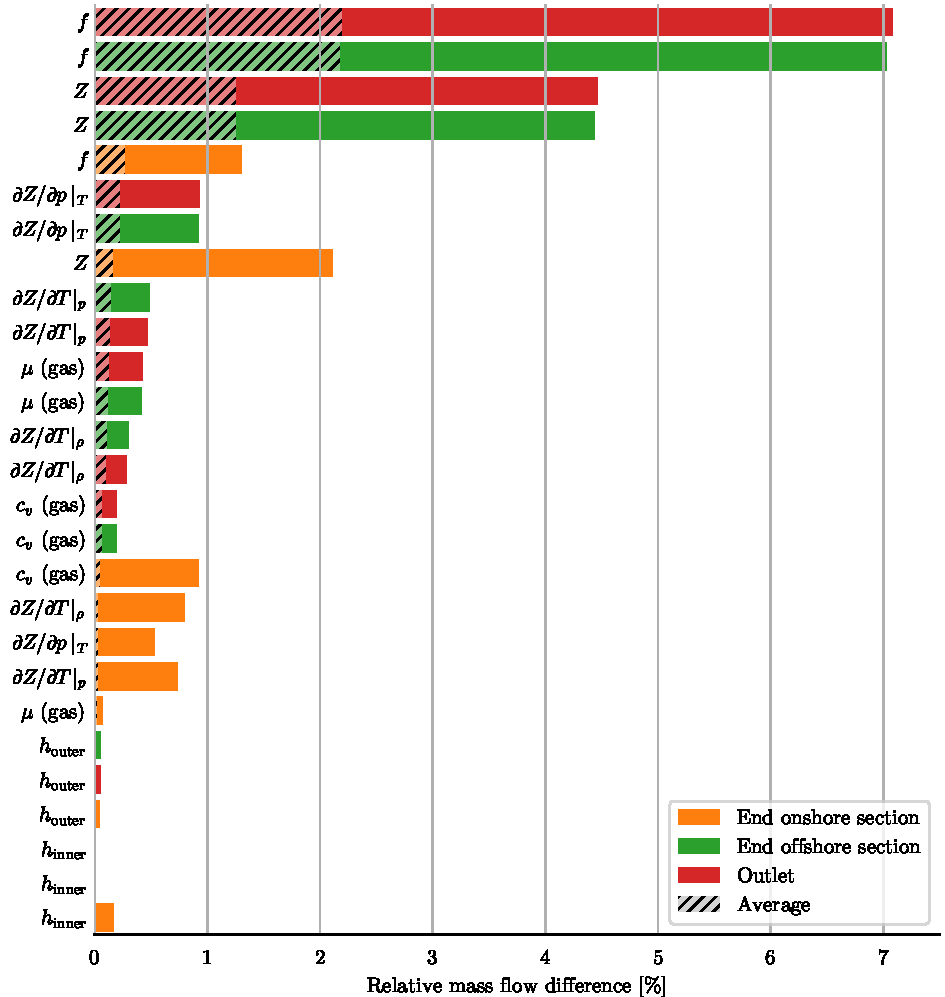
\includegraphics{figures/barchart_all_mass_flow_relative.pdf}%
%     \caption{%
%         Chart of the average and maximum relative difference in mass flow between the base case and the cases with modified parameters, for 3 different points on the pipeline (the end of the onshore section, the end of the offshore section, and the outlet). The bars are sorted by descending average error. 
%         %Only parameters/points with average relative difference above \SI{0.04}{\percent} are shown.%
%         \label{fig:massFlowBarChart}%
%     }%
% \end{figure}%

% \begin{figure}[!p]%
%     \centering%
%     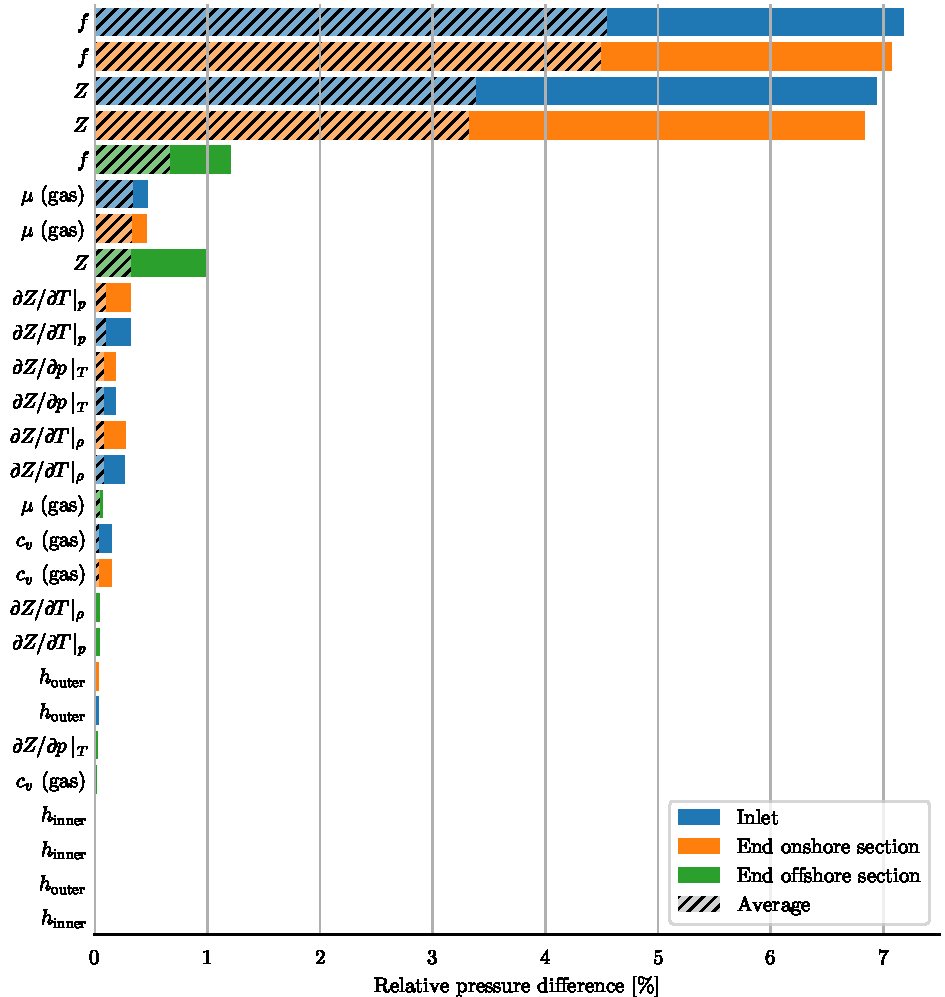
\includegraphics{figures/barchart_all_pressure_relative.pdf}%
%     \caption{%
%         Chart of the average and maximum relative difference in pressure between the base case and the cases with modified parameters, for 3 different points on the pipeline (the inlet, the end of the onshore section and the end of the offshore section). The bars are sorted by descending average error. 
%         %Only parameters/points with average relative difference above \SI{0.04}{\percent} are shown.%
%         \label{fig:pressureBarChart}%
%     }%
% \end{figure}%

\begin{figure}[!p]%
    \centering%
    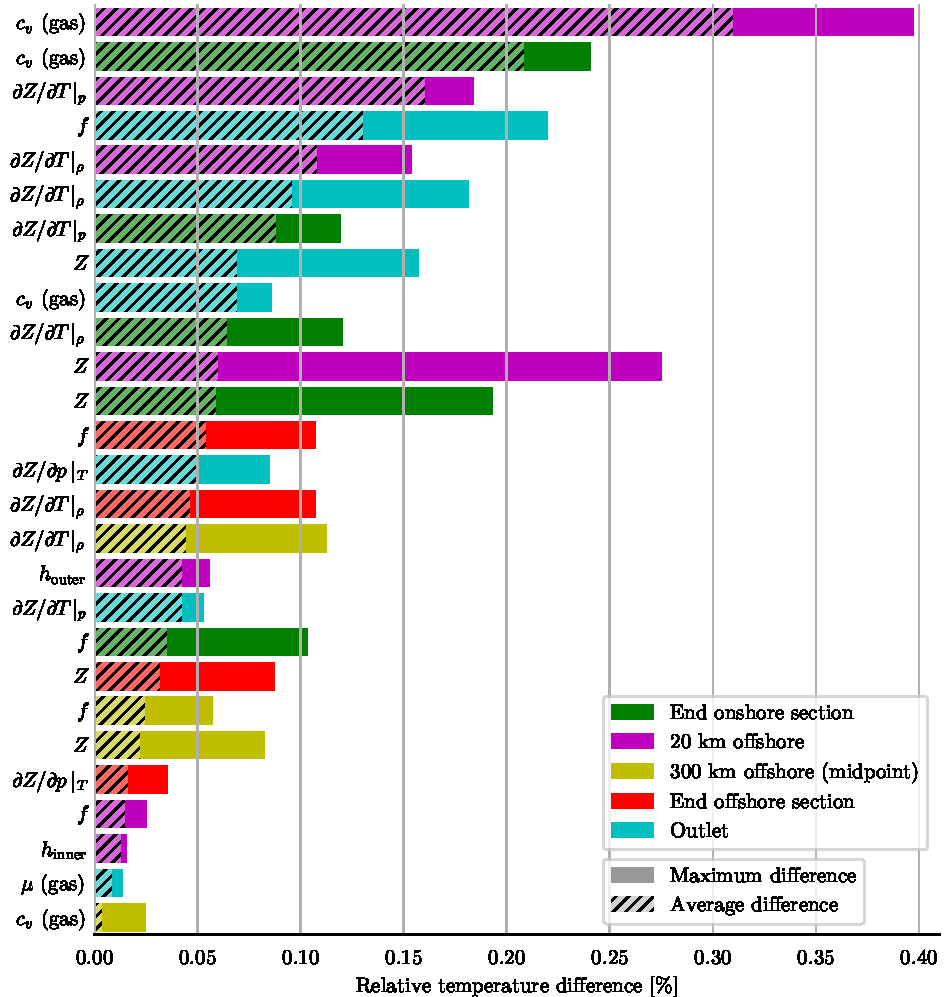
\includegraphics{figures/barchart_all_temperature_absolute.pdf}%
    \caption{%
        Chart of the average relative difference (the hatched bars) and maximum relative difference (the solid bars) in temperature between the base case and the cases with modified parameters, for 5 different points on the pipeline (the end of the onshore section, \SI{20}{\kilo\meter} off shore, \SI{300}{\kilo\meter} off shore, and the end of the offshore section). The bars are sorted by descending average error. 
        Only parameters/points with average relative difference above \SI{0.0036}{\percent} are shown.%
        % \redtext {fix figure (include average and max in legend), have good description}
        % cut-off at average absolute difference $>0.0371$ C.
        \label{fig:temperatureBarChart}%
    }%
\end{figure}%

% \begin{figure}[ht]%
%     \centering%
%     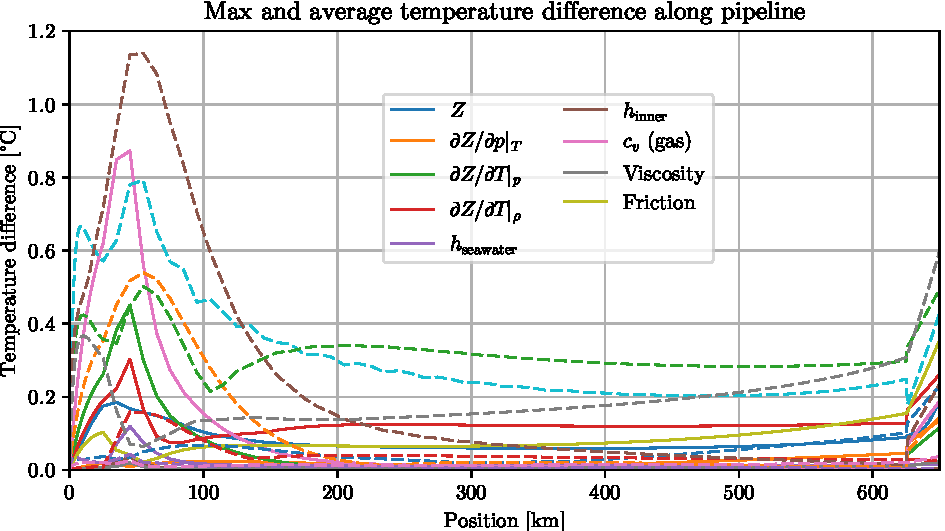
\includegraphics{figures/temperature_difference_along_pipeline.pdf}%
%     \caption{%
%         \redtext{Consider making a graph like this for mass flow and pressure as well? Could possibly make a page heigh subfigure thing.}
%         \label{fig:}%
%     }%
% \end{figure}%

% \begin{figure}[h]%
%     \centering%
%     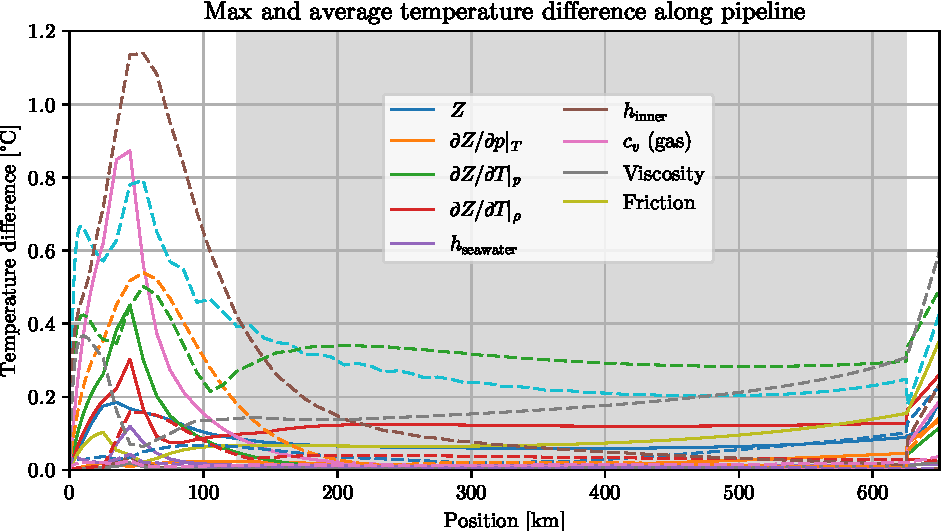
\includegraphics{figures/temperature_difference_along_pipeline_shaded.pdf}%
%     \caption{%
%         \redtext{Caption.}
%         \label{fig:}%
%     }%
% \end{figure}%